\begin{figure}[!]
\begin{center}
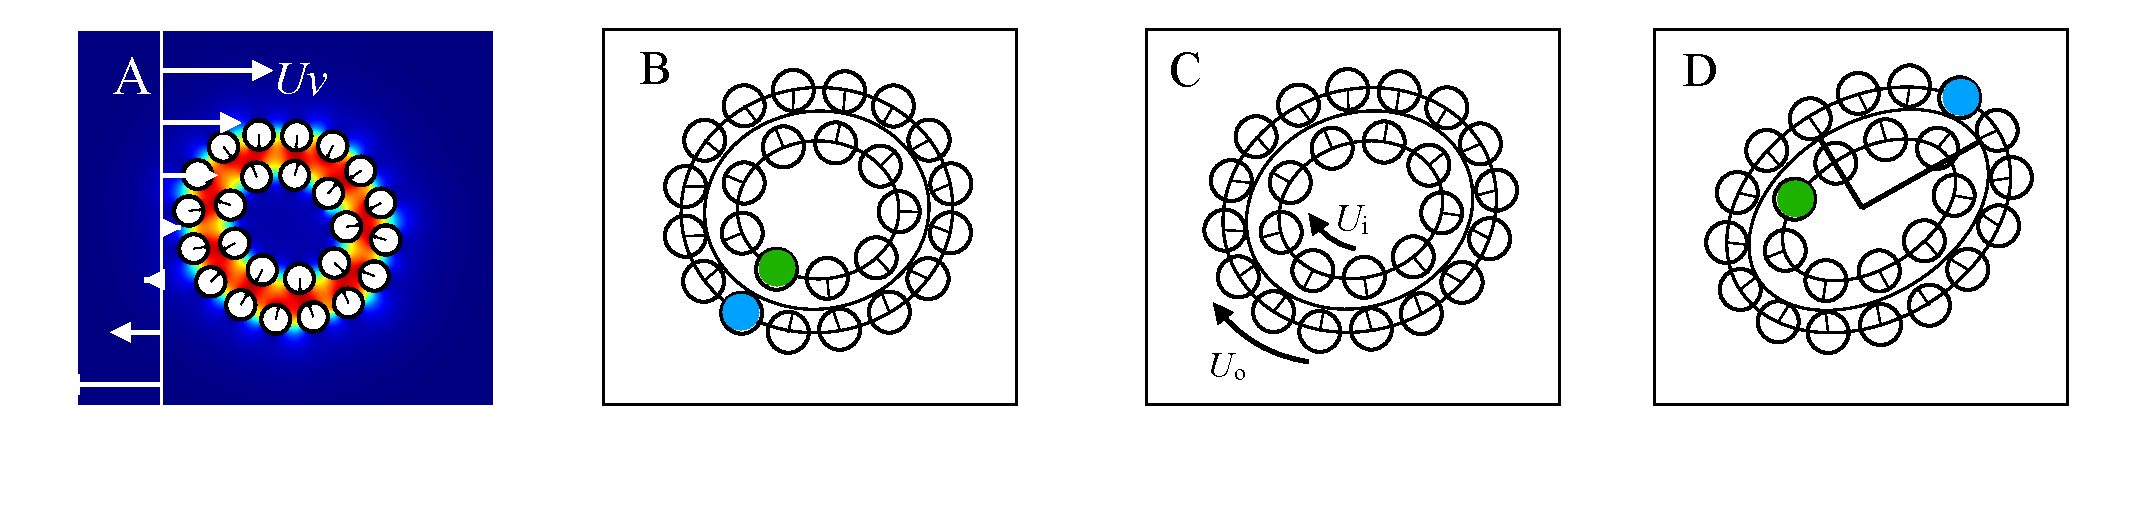
\includegraphics[width=1\textwidth]{figures/PW_fig1A-D.pdf}
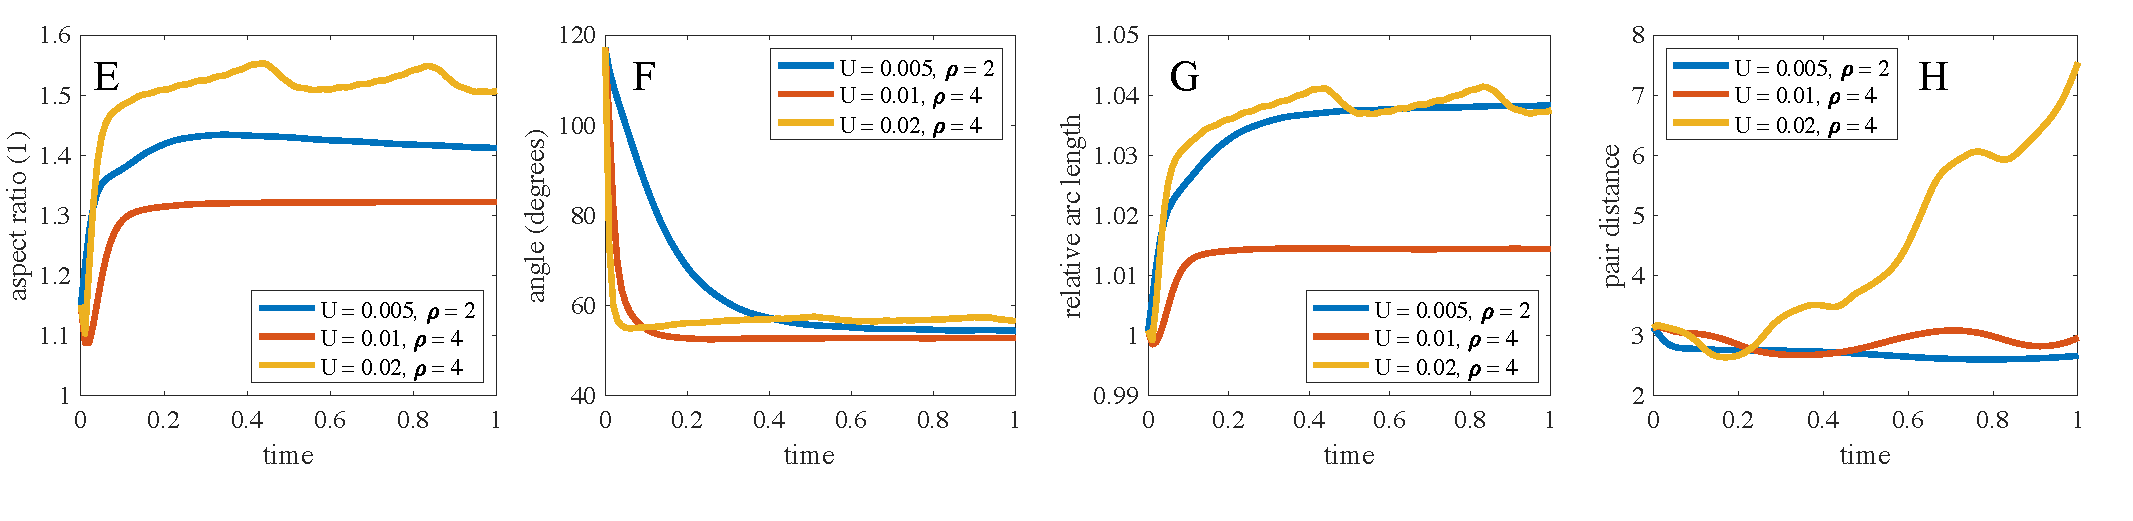
\includegraphics[width=1\textwidth]{figures/PW_fig1E-H.pdf}
\end{center}\vspace{-0.3in}
\caption{ 
(A) A vesicle formed by amphiphilic particles in shear flow,
and the tank-treading motion (B)--(D). The separation of particle
pairs in (B) and (C) illustrate inter-leaflet slip.
(E) -- (G) Tank-treading reaches a steady state in elliptical aspect ratio,
major-axis angle, and circumference. }
\label{fig:tanktreading}
\end{figure}
\section{Preliminary Work on Two-dimensional Vesicle Hydrodynamics in Shear Flow} 
%The motion of vesicles in shear flow is an important
%problem in the applied mathematics because simulations can reveal mechanical
%properties of membranes and lead to an enhanced understanding of 
%deformable particle laden flows \cite{Sinha15}. 
%
Over the past decades, researchers have used a number of mathematical tools 
to model vesicles in shear flow, including  phase field \cite{DuLiuWang2004_JCP,BibenKassnerMisbah2005_PRE}, 
level set \cite{DoyeuxGuyotChabannesEtAl2013_JCAM}, boundary integral \cite{Shravan09,Rahimian15} and 
immersed boundary approaches \cite{KimLai2010_JCP,KimLai2012_PRE,HuLaiSeolEtAl2016_JCP}. All these approaches
assume a mathematical surface, whether implicitly or explicitly, 
and define an elastic bending energy of the surface. The vesicle obeys fluid
transport and in turn the fluid balances shear stress with the vesicle's bending force. 

Our HAP approach differs from prior methods in a number of respects. 
First, we do not assume a surface. Rather, we more fundamentally  consider a collection of amphiphilic particles.
The collection of amphiphiles minimize hydrophobic interactions by sequestering hydrophobic tails in the form of a bilayer, and the particles' excess free energy gives rise to an elastic bilayer energy. 
The second difference lies in the fluid-interface coupling. Here, the associated mobility problem \eqref{eq:stokes} 
is more complicated than dealing with a stress boundary condition or diffusive surface force, 
because the fluid velocity must be that of a rigid body motion at the particle surfaces.

To implement a vesicle in shear flow in the context of hydrophobic potentials and mobility problem, 
we consider a shear flow $\mathbf{u}_{\infty} = Uy\mathbf{i}_x$ in the direction of the $x$-axis
(Figure \ref{fig:tanktreading}A).
This field satisfies the linear Stokes system but does not give rise to a rigid motion at the particle interfaces. 
To have a rigid motion, we change variables $\mathbf{u} = \tilde{\mathbf{u}}+ \mathbf{u}_{\infty}$ and 
for the new field $\tilde{\mathbf{u}}$ vanishing at infinity we let 
$\tilde{\mathbf{u}}|_{\partial P_i} = \mathbf{v}_i + \boldsymbol{\omega}_i \times (\mathbf{x} - \mathbf{a}_i)$ 
where $(\mathbf{v}_i,\boldsymbol{\omega}_i)$ are the unknown translation and angular velocities of the 
$i$th particle $P_i.$  

\begin{wrapfigure}[17]{l}{0.4\textwidth}
\centerline{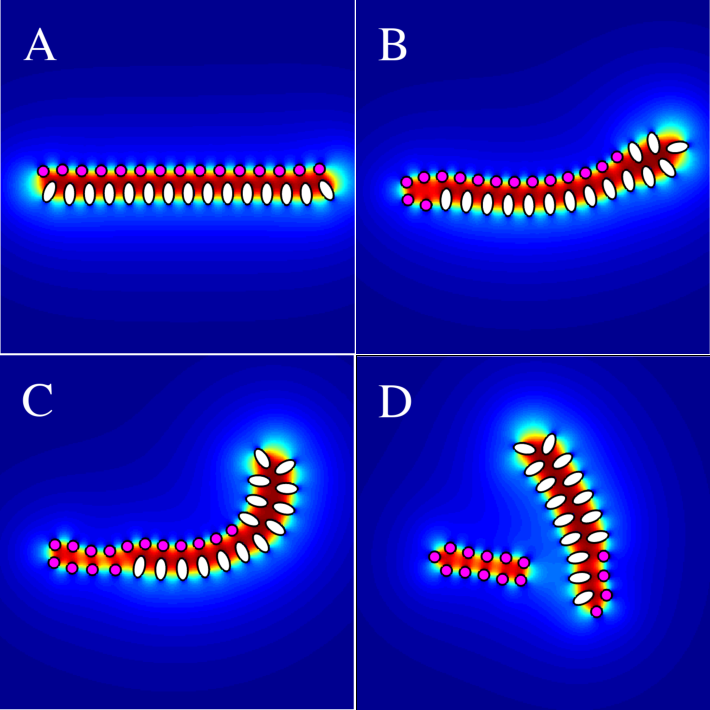
\includegraphics[width=0.4\textwidth]{figures/PW_fig2.pdf}}
\caption{\label{fig:demixing} An initial assembly of small and 
large particles spontaneous segregates into two smaller bodies. }
\end{wrapfigure}
The HAP simulations show vesicle tank-treading. Under the external shear flow, the initially circular 
vesicle rotates in the clockwise direction. As the rate of rotation increases, the vesicle approaches
a steadily tank-treading ellipse. In Figure \ref{fig:tanktreading}B-D, the solid curves are ellipses fit to the particle centers
and midplane respectively. In the non-dimensionalized system, the particles have diameter 2, on the order of $\rho,$ 
and the vesicle diameter is about 14. 
Figure \ref{fig:tanktreading}E shows the aspect ratio of the major to minor axes reaching an equilibrium value in the 
red and blue curves, yet oscillating in the high-shear rate (yellow) curve.
The tank-treading vesicle elongates and becomes more horizontal 
with an increase in flow rate or 
with a decrease in stiffness (effected by decreasing $\rho = 4$ to $\rho = 2$). 



For large shear flow rates, there is an increase in arc length. Here arc length
refers to the the mid-plane circumference. Thus,
some of the external force is going into stretching the vesicle--the other
part is going into bending and viscous dissipation. From our experiments, 
we find that the vesicle ruptures once stretching exceeds about 5 \%
(see Figure \ref{fig:rupture}).
Finally, movies of the tank-treading motion show a slip velocity
between the outer and inner leaflets Figure \ref{fig:tanktreading}G. We have illustrated this 
by tracking the distance between two reference particles in the inner and outer leaflet
(Figure \ref{fig:tanktreading}B \& D, green and blue particles). 
With moderate shear rates or greater adhesion, the particle pair moves in tandem
(in Figure \ref{fig:tanktreading}H, blue and red curves, their distance is more or less constant). 
For a large shear rate, the particle separates as the two leaflets slide against one another. 



\begin{wrapfigure}[12]{r}{0.2\textwidth}
\centerline{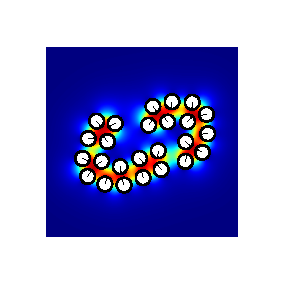
\includegraphics[width=0.2\textwidth]{figures/PW_fig5.pdf}}
\caption{\label{fig:rupture} Rupture of tank-treading vesicle under strong shear flow.}
\end{wrapfigure}
There are a number of advantages to using our particle based approach.
For one, the HAP theory automatically accounts for the existence of multiple phases. 
For example, we can vary lipid length, spontaneous curvature and bending rigidity 
by introducing differentiating particle shapes and hydrophobic boundary conditions (Figure \ref{fig:demixing}).
Continuum theory deals with multiple phases through additional surface densities that must
then satisfy specialized transport equations \cite{Lowengrub07,MikuckiZhou17}. 
As illustrated in Figure \ref{fig:tanktreading}, the particle
based approach supports inter-leaflet slip, and this can be used to determine inter-leaflet
and in-plane shear viscosities. 





The ability to form discontinuities is perhaps the HAP method's greatest 
strength. Indeed, a strong, extensional shear flow must cause membrane rupture since the 
energy of stretching must exceed the pore nucleation and widening barriers 
for sufficiently large flow strengths. 
Some disadvantages are that the hydrophobic interaction does not constrain vesicle volume. 
Instead, changes in volume are rate limited by inter-particle spacing,
which may be undesirable in case of a mathematically strict volume constraint.
% set vesicle volume, as is done in the study of liposomes
%using auxiliary constraint equations for instance. 
%Also, the boundary integral method formulation
%relies on linearity of the Stokes equations. There has been some progress in
%boundary integral methods for the non-linear Navier-Stokes equations [ref].
%We point out that some non-Newtonian effects in polymers are a consequence of hydrophobic
%and steric molecular interactions like the ones presented in this proposal. 

In recent years, researchers have developed a number of numerical methods for calculating
energy minimizing steady equilibrium shapes of lipid bilayer membranes, vesicles and red blood cells.
These approaches range from the finite element method~\cite{Bartels,Peng13,RyKlYaCo16,Sinha15}, 
phase field method \cite{Du05,QiangDu08,Lowengrub13} to immersed boundary method  \cite{Hu,Hu13, Kim10}.
PI Ryham and collaborators led in part the development of phase field
functionals of membrane elastic energy and approaches to coupling membrane elasticity to fluids  \cite{0951-7715-18-3-016,Du05,DuEuler,QiangDu09}.

